\documentclass{paper}
\usepackage[utf8]{inputenc}
\usepackage[titles]{tocloft}
\renewcommand{\cftdotsep}{1}
\usepackage{graphicx}
\usepackage[dvipsnames]{xcolor}
\definecolor{background_blue}{HTML}{e3f3ff}  
\usepackage[a4paper, total={6in, 9.5in}]{geometry}
\usepackage{titlesec}

\titleformat*{\section}{\LARGE\bfseries}
\titleformat*{\subsection}{\Large\bfseries}
\titleformat*{\subsubsection}{\large\bfseries}
\titleformat*{\paragraph}{\large\bfseries}
\titleformat*{\subparagraph}{\large\bfseries}
\begin{document}
\pagestyle{plain}
\begin{titlepage}
	\centering
	
	\vspace{2.5cm}
	{\huge\bfseries Fides\par}
	\vspace{1cm}
  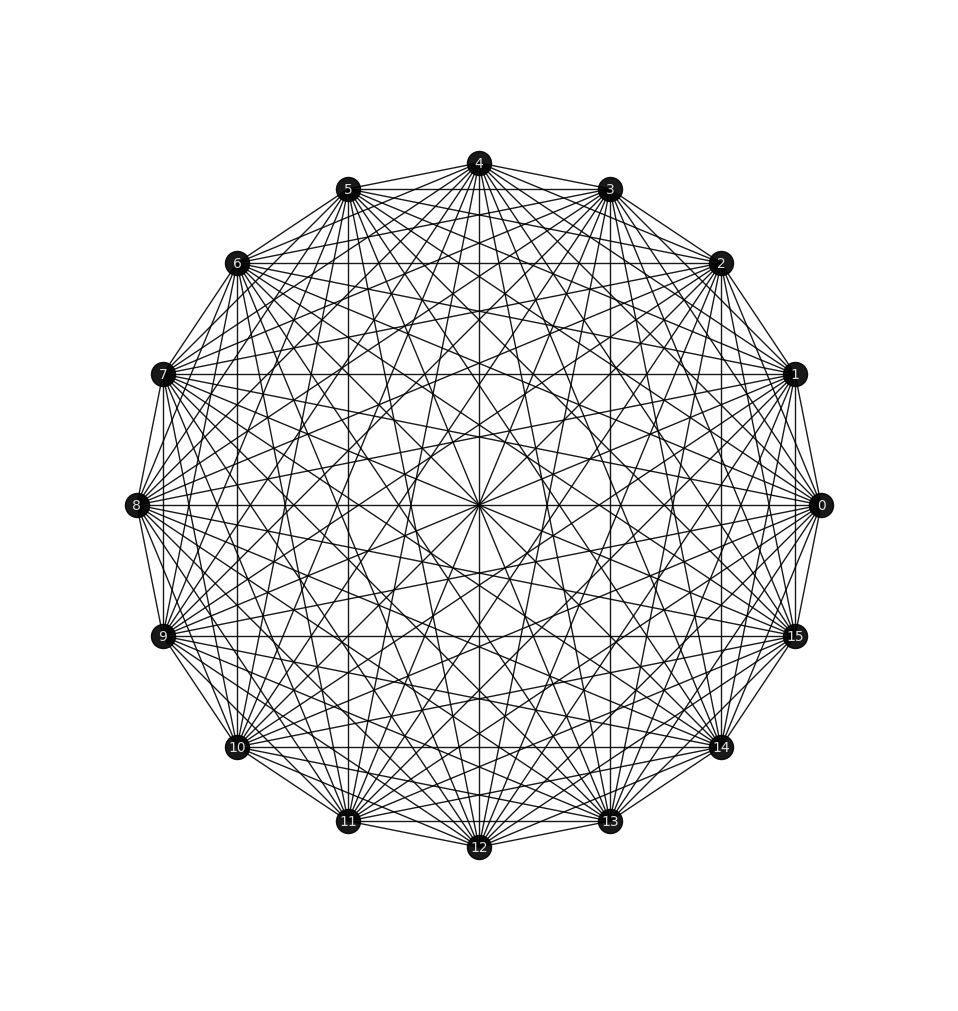
\includegraphics[width=0.5\textwidth]{16_nodes_fully_connected.png}\par\vspace{1cm}
	{\Large\itshape Experimental multi party web hosting solution\par\vspace{1cm}}


  \par\vspace{1cm}
% Bottom of the page
	{\large \today\par}
\end{titlepage}

\title{Fides}
\tableofcontents
\newpage

\section{Introduction}

Dapps these days are primarly accessed via websites. These websites are very often hosted on a single server or cluster, controlled by very few parties. Furthermore, these websites largely cannot be held accountable for the information they provide, because almost none of them use any kind of signature scheme. The teams behind dapps are not incentived to improve this situation : it's cheaper and more convenient to host a website "the traditionnal way". Users of these dapp's do not seem to care either : they just want a fast, reliable and convenient website. 
\\\\
The Fides system aims to make the relationship between the dapp's user and the server that gives critical information (asset prices, verified tokens, etc...) more trustless and robust; while remaining convenient to implement for both the users and the dapp developers.
\\\\
From the user perspective, Fides is just another open source web browser extension, easily installable from a browser store or from source. Once installed, there is no setup required.
\\\\
From the dapp developer perspective, Fides is a simple reverse-proxy, with a full Ergo node and wallet attached. The developers just need to put the Fides reverse-proxy in front of their existing servers, setup the wallet and operate as usual.

\section{Cryptography}

\section{Description of the Fides system}

\subsection{Cell}

A Cell is composed of a domain name, a private key to a wallet with staked tokens, the Fides nodes serving static files and connected to a redis database and an Ergo full node.

\subsection{Registration}
To register, a cell must send an amount of the DAO's tokens, with the domain name in the metadata

\subsection{Initialisation}
Once registered, the cell download the UI, the data, etc... from other nodes if they exist. We call this \i{cell duplication}. If it's the first node (we can see that if it's the first utxo in the smart contract), the cell can have arbitrary UI, data, etc...

\subsection{Consensus}
Cells check each other's work : e.g. if cell A,B,C respond the value "X" to the get request G, but cell D and E respond "Y" to G; A, B or C can report the faulty cells to the SC.
\\
If the majority of the cells then signs the report (by interacting with the SC with their stacked wallet), the staking rewards of the faulty cells are put 50\% into the reporting cell, the other 50\% are distributed among the cells that co-signed the report.

\subsection{Responses and requests signatures}
Responses of cells are always signed, meaning the reports are tamper-proof : the reporting cell can prove with certainty that the faulty cell misbehaved. The faulty response, along with the signature, is send to the smart contract which then verify the report. The signatures also prevent cells  being reverse-proxies : a cell cannot just pass the request to another cell, because the response will be signed by the cell that actually fulfilled the request.
\\

Request from cells are also signed, meaning if a cell harass another cell, the spam victim can report the harasser and get his staking rewards.

\subsection{Architecture overview}

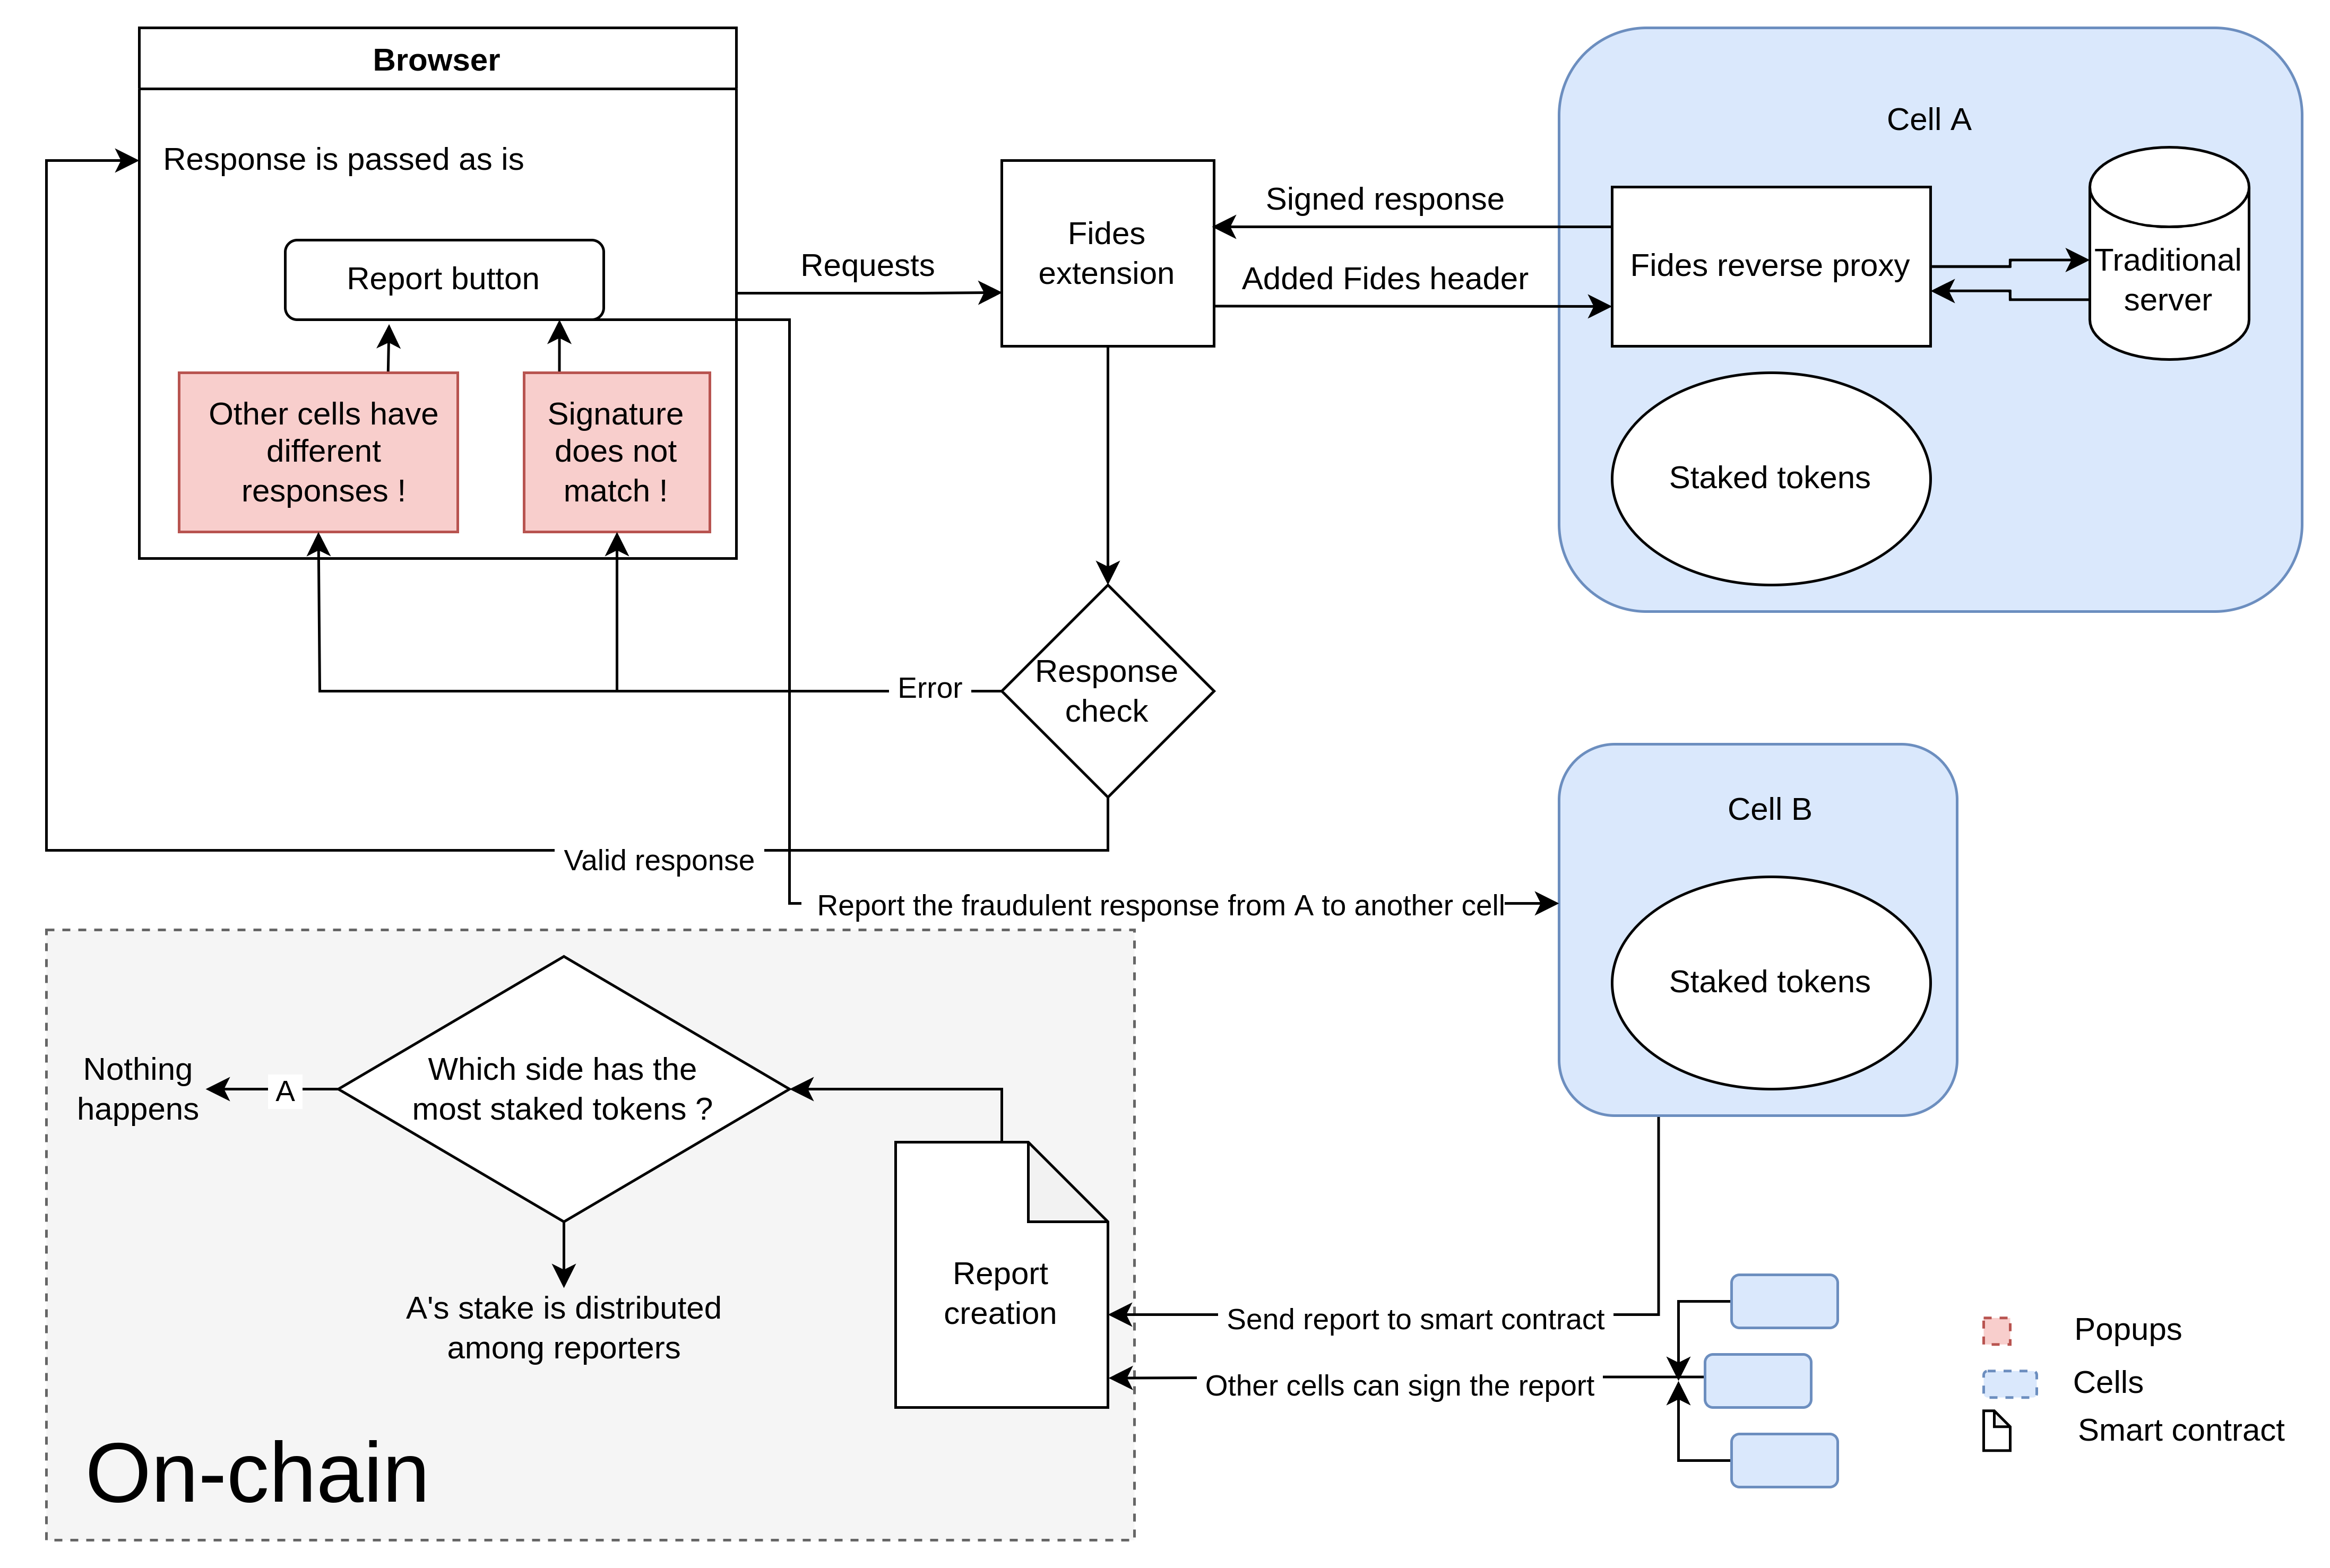
\includegraphics[width=\textwidth]{fides_flowchart.png}\par\vspace{1cm}

\subsection{Defining misbehaviour}
6. A difference is made between new data, which could lag a little between participants, and old data (5 minutes old or more) and static assets (UI components : images, .css, etc...). non consensus on very new data is not punished, only old data and static assets can make a potentially valid report

7. Every time a cell A makes a request to another cell B, A tells every other cell. That way, if B is just passing the request to another cell C (e.g. by being a more sophisticated reverse proxy, that reads the content of responses, and sign them using his private key), C can report B for leeching on the system : B collects staking rewards but does not contribute because it's not a real server.

\section{Limitations and principles}

\section{Implementation proposition}
\end{document}